\documentclass[a4paper,10pt]{article}
\usepackage[utf8]{inputenc}
\usepackage[english]{babel}

\usepackage[backend=bibtex8]{biblatex}
\bibliography{./../final_project_sources}

\usepackage{graphicx}
\usepackage{caption}

\usepackage{multirow}
\usepackage[table,xcdraw]{xcolor}

\usepackage{mathtools}
\usepackage{bm}
\usepackage{textcomp}

\usepackage[linesnumbered,ruled]{algorithm2e}

% Title Page
\title{Biotech Beer Brewing\\Project status report}
\author{Dominik Schmidt\\Jakob Wittmann}

\begin{document}
\maketitle

%\begin{abstract}
%\end{abstract}

\section{Project status}

% To-Do:
% \begin{itemize}
%  \item Start with introduction of processes, the figure with the project timeline does not point out the processes well enough
%  \item update table ``project processes''
%  \item update figure ``project progress''
%  \item update text in this section
% \end{itemize}


\subsection{Milestones}

\begin{figure}[h]
 \centering
 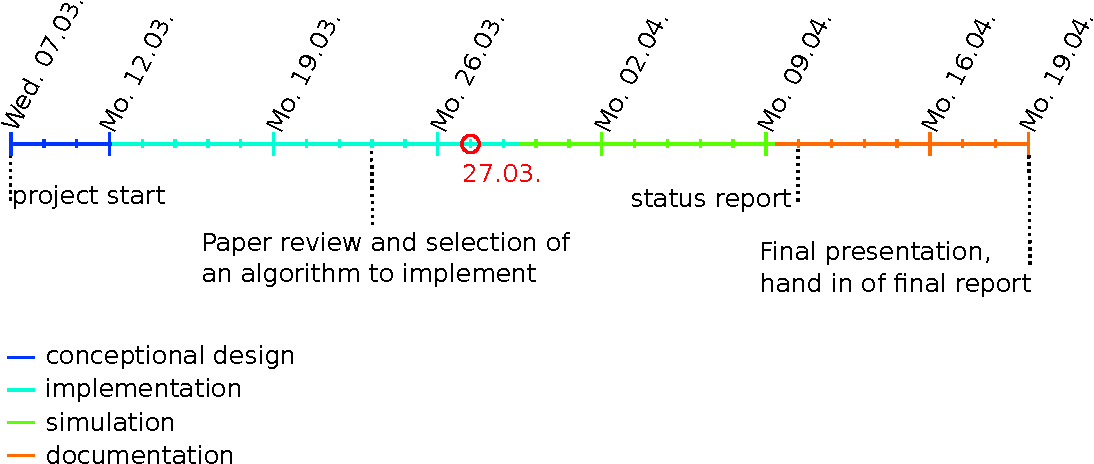
\includegraphics[width=\linewidth]{timeline.pdf}
 \caption{Project timeline}
 \label{fig:project_timeline}
\end{figure}

\begin{table}[h]
\centering
\caption{Project processes}
\label{tab:project_processes}
\begin{tabular}{llllll}
\rowcolor[HTML]{EFEFEF} 
\cellcolor[HTML]{EFEFEF}                          & \multicolumn{2}{c}{\cellcolor[HTML]{EFEFEF}Effort} & \cellcolor[HTML]{EFEFEF}                             & \cellcolor[HTML]{EFEFEF}             &      \\
\rowcolor[HTML]{EFEFEF} 
\multirow{-2}{*}{\cellcolor[HTML]{EFEFEF}Process} & Days                  & Percent                   & \multirow{-2}{*}{\cellcolor[HTML]{EFEFEF}start date} & \multirow{-2}{*}{\cellcolor[HTML]{EFEFEF}due date} & \multirow{-2}{*}{\cellcolor[HTML]{EFEFEF}progress} \\
conceptional design                               & 3.1 d   & 10 \%  & 07.03. & 12.03. & 100 \% \\
implementation                                    & 12.4 d  & 40 \%  & 12.03. & 28.03. & 92 \% \\
\hspace{0.5cm}research                            & 4.65 d  & 15 \%  & 12.03. & 16.03. & 100 \% \\
\hspace{0.5cm}concept                             & 1.55 d  & 5 \%   & 16.03. & 20.03. & 100 \% \\
\hspace{0.5cm}coding                              & 6.2 d   & 20 \%  & 20.03. & 28.03. & 75 \% \\
simulation                                        & 7.75 d  & 25 \%  & 28.03. & 09.04. & 42 \% \\
\hspace{0.5cm}research                            & 4.65 d  & 15 \%  & 28.03. & 30.03. & 75 \% \\
\hspace{0.5cm}setup                               & 1.55 d  & 5 \%   & 30.03. & 02.04. & 50 \% \\
\hspace{0.5cm}simulate setup                      & 1.55 d  & 5 \%   & 02.04. & 09.04. & 0 \% \\
documentation                                     & 7.75 d  & 25 \%  & 09.04. & 17.04. & 0 \% \\
\hspace{0.5cm}analyze results                     & 1.55 d  & 5 \%   & 09.04. & 10.04. & 0 \% \\
\hspace{0.5cm}prepare presentation                & 3.1 d   & 10 \%  & 10.04. & 16.04. & 0 \% \\
\hspace{0.5cm}prepare report                      & 3.1 d   & 10 \%  & 16.04. & 17.04. & 0 \% \\
\end{tabular}
\end{table}

\subsection{Progress}

\begin{figure}[h!]
 \centering
 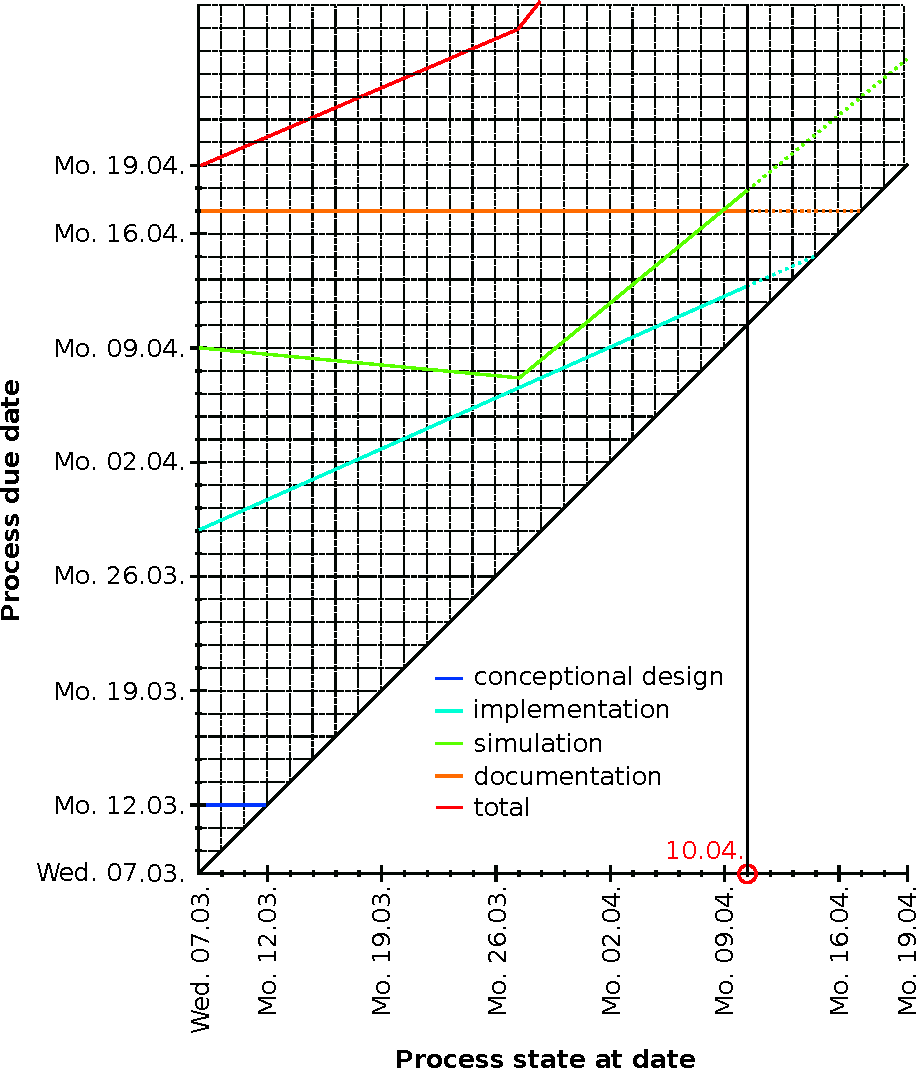
\includegraphics[width=\linewidth]{progress.pdf}
 \caption{Project progress}
 \label{fig:project_progress}
\end{figure}

The progress of the main project processes in table \ref{tab:project_processes} is illustrated in figure \ref{fig:project_progress}. 
The dashed colored lines show a simple estimated future progress of the processes. If the current trend holds on, the project will be
finished approximately 26 working days after the final due date.


\newpage

\section{Presentation of intermediate results}
\subsection{Simulation algorithm}

This project will use parts of the Dynamic Multispecies Metabolic Modeling (DMMM) framework to implement dynamic flux balance analysis
(DFBA). Table \ref{tab:overview_implemented_features_compared_to_dmmm} compares selected features of the original implementation of DMMM
with the implementation in this project.

\begin{table}[h]
\centering
\caption{Overview of implemented features compared to DMMM}
\label{tab:overview_implemented_features_compared_to_dmmm}
\begin{tabular}{llllll}
\rowcolor[HTML]{EFEFEF} 
\cellcolor[HTML]{EFEFEF} Feature                  & \cellcolor[HTML]{EFEFEF}DMMM & \cellcolor[HTML]{EFEFEF}This project\\
Model                                    &   &  \\
\hspace{0.5cm}arbitrary many GEMs & yes & yes \\
\hspace{0.5cm}\begin{tabular}[c]{@{}l@{}}arbitrary many metabolites\\ in environment\end{tabular} & yes & yes \\
\hspace{0.5cm}mortablility of bacteria & \begin{tabular}[c]{@{}l@{}}yes\\(in output flux)\end{tabular} & yes \\
\hspace{0.5cm}\begin{tabular}[c]{@{}l@{}}input/output flux of bacteria\\ and metabolites\end{tabular} & yes & no \\
\hspace{0.5cm}\begin{tabular}[c]{@{}l@{}}parameterized initial state\\ of environment composition\end{tabular} & yes & yes \\
\hspace{0.5cm}Michaelis-Menten kinetics & yes & yes \\
Algorithm &  &  \\
\hspace{0.5cm}ODE solver & yes & yes \\
\hspace{0.5cm}different ODE solvers & yes & no \\
\hspace{0.5cm}analytical solver & yes &no \\
\end{tabular}
\end{table}

%Content:
%\begin{itemize}
% \item Show the used theorys behind DMMM
% \begin{itemize}
%  \item Differential equations
%  \item Michaelis-Menten kinetics
%  \item Mortality
%  \item including units
% \end{itemize}
%
% \item for the basics refer to DMMM papers:
% \begin{itemize}
%  \item Formulas: \cite{zhuang_design_2012}
%  \item Implementation: \cite{zhuang_genome-scale_2011}
% \end{itemize}
% 
% \item Show implementation as pseudocode
%\end{itemize}

% Open Questions:
% \begin{itemize}
% % \item How to model mortality?
% % \item How did Zhuang implement it?
%  \item How to determin the actual input and output fluxes of the GEMs in one timestep? - What did Zhuang do?
% \end{itemize}

As described by Zhuang et al. in \cite{zhuang_genome-scale_2011} the algorithm uses a ODE solver with embedded FBA. A FBA is solved
for each GEM in the model and for each time step in the discretised simulation time interval considering the changed metabolite and
bacteria densities in the shared environment. The results of the FBAs are used by the ODE solver to solve the differential equations

\begin{equation} \label{eq:diff_eq_x}
 \frac{\mathrm d x_j}{\mathrm d t} = \mu_j x_j
\end{equation}
\begin{equation} \label{eq:diff_eq_s}
 \frac{\mathrm d s_i}{\mathrm d t} = \displaystyle\sum_{j=1}^{N} v_{i,j} x_j
\end{equation}

which models the dynamics of the bacteria's environment \cite{zhuang_design_2012} where $i = 1...N$ is the index of metabolites in the shared environment and $j = 1...M$ is the index of bacteria.
The bacteria density is modeled in $x_j$ with $\left[ x_j \right] = \frac{g}{l}$ and $\mu_j$ is the bacteria's growth rate with $\left[ \mu_j \right] = \frac{mmol}{g_{DW} h}$.
Input and output fluxes of the bacteria's models are modeled in $v_{i,j}$ with $\left[ v_{i,j} \right] = \frac{mmol}{g_{DW} h}$,
the densities of metabolites in the shared environment in $s_i$ with $\left[ s_i \right] = \frac{mmol}{l}$.

In each time step each bacteria's metabolite intake must be changed dependent on the densities of the metabolites in the shared environment.
To model saturation of metabolite intake for high metabolite densities Zhuang et al. implemented Michaelis-Menten kinetics \cite{johnson2011original}

\begin{equation} \label{eq:michaelis-menten}
 v_{max,i,j} = \frac{v_{mm,i,j} s_i}{s_i + k_{mm,i,j}}
\end{equation}

This formula describes the upper bound of the input flux $v_{max,i,j}$ for metabolite i of bacteria j dependent on the metabolite density
$s_i$. The formula is characterized by to constants $\left[ v_{mm,i,j} \right] = \frac{mmol}{g_{DW} h}$ and $\left[ k_{mm,i,j} \right] = \frac{mmol}{l}$
for each bacteria and metabolite.

Mortality is considered using a constant $\left[ \mu_{mort,j} \right] = \frac{mmol}{g_{DW} h}$ for each bacteria j in this implementation while Zhuang et al. modeled this
using the output flux of bacteria out of the system.

%To-Do:
%\begin{itemize}
% \item mortabilität einbauen: Welches modell nehme ich dafür? Absterben falls growth geht gegen 0? Oder eine Mortabilität als faktor?
% \item Vergleiche $V_{max}$ und K mit geweiligen Paper und checke ob die Gleichungen stimmen
% \item Schreibe bisschen was zu den Michaelis-Menten kinetics
% \item Male ein Bild das die Simulation darstellt (evtl. ähnlich wie im DMMM paper?)
% \item giesse die Optimierung in eine mathematische Beschreibung
% \item erstelle Pseudocode um den Algorithmus zu beschreiben
%\end{itemize}

Algorithm \ref{alg:differential_equation_with_embedded_fba} shows a basic implementation of the differential equations solved by an ODE
solver during the simulation similar to DMMM \cite{zhuang_genome-scale_2011}.

The algorithm expects a list of bacteria models consisting of
\begin{itemize}
 \item GEM of this bacteria: A, $\bm{v_{min}}$, $\bm{v_{max}}$, $\bm{w_{growth}}$
 \item $\bm{v_{mm}}$ (Michaelis-Menten $V_{max}$) for each exchange metabolite and species
 \item $\bm{k_{mm}}$ (Michaelis-Menten K) for each exchange metabolite and species
 \item mortality $\mu_{mort}$
\end{itemize}

Furthermore a list of all exchange metabolites in the environment, the bacteria and metabolite densities.


\begin{algorithm}
    \SetKwInOut{Input}{Input}
    \SetKwInOut{Output}{Output}

    \underline{function step}$(model_1...model_M, m_1...m_N, x_1...M, s_1...s_N)$\;
    \Input{bacteria models $model_j$, exchange metabolites $m_i$ in environment, bacteria densities $x_j$, metabolite densities $s_i$}
    \Output{slope of bacteria and metabolite densities $\dot{x}_j, \dot{s}_i$}
    \For{$j := 1$ \KwTo M}{
      \For{$i := 1$ \KwTo M}{
%	$\bm{v_{max,j}}[m] := michaelis\_menten(\bm{vmm_{j}}[m], \bm{kmm_{j}}[m], s[m])$
	$model_j := update\_intake\_bounds(model_j, s_j, m_i)$
      }
    }
    \For{$j := 1$ \KwTo M}{
      $\mu_j, \bm{v_j} := FBA(model_j, \bm{w_{growth}})$
    }
    $\bm{\mu} := \bm{\mu} - \bm{\mu_{mort}}$\\
    $\dot{\bm{x}} := diag(\bm{\mu}) \, \bm{x}$\\
    \For{$j := 1$ \KwTo M}{
      \For{$i := 1$ \KwTo N}{
        $\bm{\dot{s}}[m_i] := \bm{\dot{s}}[m_i] + \bm{v_j}[m_i] x_j$
      }
    }
    return $\dot{\bm{x}}$, $\dot{\bm{s}}$
    \caption{Differential equation with embedded FBA}
    \label{alg:differential_equation_with_embedded_fba}
\end{algorithm}

In a first step the upper bounds of the intake fluxes are updated for each bacteria j and exchange metabolite i.
The function $update\_intake\_bounds(model_j, s_j, m_i)$ calculates the upper bounds using the formula \ref{eq:michaelis-menten} if
the metabolite $m_i$ is contained in $model_j$ as a exchange metabolite and updates this value in the model.

In a next step the GEMs are optimized for growth using FBA, the results are used as growth rate $\mu_j$ and actual input and output
fluxes $\bm{v_j}$ of bacteria j in this time step.

The mortality is considered by subtracting the constants $\bm{\mu}$ from the growth rates $\bm{\mu}$.

At last step the slopes $\dot{\bm{x}}$ and $\bm{\dot{s}}$ are calculated according to \ref{eq:diff_eq_x} and \ref{eq:diff_eq_s} and
returned to the ODE solver.

\subsection{Simulation Setup}

% \begin{itemize}
%  \item used GEMs
%  \item why did we choose them? - Is there a reason??
%  \item Simulation parameters: $V_{max}$, K, mortality
%  \item How should the simulation be done?
%  \begin{itemize}
%   \item what are the ``simulation parameters''?
%   \item what do we want to measure?
%   \item What do we want to show?
%   \begin{itemize}
%    \item The simulator works
%    \item Capabilities of this simulations (usage in later applications)
%   \end{itemize}
%  \end{itemize}
% \end{itemize}

The goal of the simulation is to validate the basic functionality of the simulator using a simplified setup of a realistic future
simulation scenario. As defined in our project goals, this simulation scenario is the dynamic flux balance analysis (DFBA) of a
co-culture of Saccharomyces cerevisiae and Lactobacillus plantarum.

As genome-scale models a model of Lactobacillus plantarum published by Teusink et al. \cite{teusink_analysis_2006}. A decision about
a yeast model is not made yet.

The simulation will consider two input metabolites: oxygen and glucose. Table \ref{tab:model_constants_simulation_setup} and table
\ref{tab:simulation_parameters_simulation_setup} contain all values needed to define the initial metabolite conditions and kinetics.

\begin{table}[h]
\centering
\caption{Model constants used in the simulation setup}
\label{tab:model_constants_simulation_setup}
\begin{tabular}{llllll}
\rowcolor[HTML]{EFEFEF} 
\cellcolor[HTML]{EFEFEF} Constant          & \cellcolor[HTML]{EFEFEF}S. cerevisiae & \cellcolor[HTML]{EFEFEF}L. plantarum\\
Maximum glucose uptake rate (mmol/g/h)     & 18.5 & ? \\
Maximum oxygen uptake rate (mmol/g/h)      & 2.5 & ? \\
Glucose uptake saturation constant (g/l)   & 0.5 & ? \\
Oxygen uptake saturation constant (mM)     & 0.005 & ? \\
\end{tabular}
\end{table}


% \begin{itemize}
%  \item Input metabolites:
%  \begin{itemize}
%   \item Oxygen
%   \begin{itemize}
% %   \item oxygen saturation of water at 20\textdegree C = 9.077 $\frac{mg}{l}$ \cite{fao_water_1987}
% %   \item $s_{init} = 9.077 \frac{mg}{l} = 9.077 \,\, 10^{-3}  \frac{g}{l} = \frac{9.077 \,\, 10^{-3} \frac{g}{l}}{18.015 \,\, 10^{-3} \frac{g}{mmol}} = 0,5039 \frac{mmol}{l}$
% %   \item $V_{max,lac} = ?$
% %   \item $k_{m,lac} = ?$
% %   \item $V_{max,sac} = 2.5 \frac{mmol}{g \,\, h}$ \cite{hanly_dynamic_2014}
% %   \item $k_{m,sac} = 0.005 mM$ \cite{hanly_dynamic_2014}
%   \end{itemize}
%   \item Glucose
%   \begin{itemize}
% %   \item $s_{init}$: 5...20 \textdegree Plato $= 153.031...690.697 \frac{mmol}{l}$
% %   \item \cite{bubnik1995sugar}
% %   \item $V_{max,lac} = ?$
% %   \item $k_{m,lac} = ?$
% %   \item $V_{max,sac} = 18.5 \frac{mmol}{g \,\, h}$ \cite{hanly_dynamic_2014}
% %   \item $k_{m,sac} = 0.5 mM$ \cite{hanly_dynamic_2014}
%   \end{itemize}
%  \end{itemize}
%  \item Output metabolites (considered in results):
%  \begin{itemize}
%   \item ethanol
%   \item D lactate (R\_EX\_lac\_D\_e\_ in model)
%   \item L Lactate exchange (R\_EX\_lac\_L\_e\_ in model)
%  \end{itemize}
% 
% 
% \end{itemize}







\begin{table}[h]
\centering
\caption{Simulation parameters used in the simulation setup}
\label{tab:simulation_parameters_simulation_setup}
\begin{tabular}{llllll}
\rowcolor[HTML]{EFEFEF} 
\cellcolor[HTML]{EFEFEF} Parameter          & \cellcolor[HTML]{EFEFEF}value & \cellcolor[HTML]{EFEFEF}reference\\
Initial glucose density (mmol/l) & 272.9 ... 1230.755 & equation \ref{eq:ready_to_use_plato_to_metabolite_density}, table \ref{tab:constants_used_in_this_document} \\
Initial oxygen density (mmol/l)  & 0.5039 & equation \ref{eq:init_oxygen_density}, table \ref{tab:constants_used_in_this_document}\\
\end{tabular}
\end{table}

To verify the basic functionality of the simulator the resulting bacteria densities and metabolite densities of ethanol, d- and l-lactate,
oxygen and glucose will be compared to existing data.

\section{Outlook}

The current delay of 26 days will be compensated with additional shifts and it is assumed that parts of both status reports can be reused
in the final report.

\vspace{0.5cm}
The subsequent steps include:
\begin{itemize}
 \item debugging of simulator code
 \item research on metabolite kinetics for Lactobacillus plantarum
 \item choosing a yeast GEM
 \item research on reference data to verify simulation results
 \item start simulations
\end{itemize}

\section{Appendix}

The following approximation is used to convert \textdegree C (``degree plato'') to a density measure (g/l)\cite{bubnik1995sugar}.
\begin{equation} \label{eq:grad_plato_to_density}
 d_{total} = 4.13 \frac{g}{l \,\,\, ^\circ P} p + 997 \frac{g}{l}
\end{equation}

As the simulation framework expects metabolite densities relative to the total volume of the solution (mmol of metabolite per liter
solution, mmol/l) the total density $d_{total}$ must to converted to a density $s_{glc}$. It is assumed that $V_{total} = V_{glc} + V_W$.

\begin{equation*}
 d_{total} = \frac{m_{total}}{V_{total}}
\end{equation*}
\begin{equation*}
 d_{total} = \frac{m_{glc} + m_w}{V_{total}}
\end{equation*}
\begin{equation*}
 d_{total} = \frac{m_{glc} + d_w V_w}{V_{total}}
\end{equation*}
\begin{equation*}
 d_{total} = \frac{m_{glc} + d_w \left(V_{total} - V_{glc}\right)}{V_{total}}
\end{equation*}
\begin{equation*}
 d_{total} = \frac{m_{glc} + d_w \left(V_{total} - \frac{m_{glc}}{d_{glc}}\right)}{V_{total}}
\end{equation*}
\begin{equation} \label{eq:total_density_to_metabolite_density}
 s_{glc} = \frac{m_{glc}}{V_{total}} = \frac{d_{total} - d_w}{1 - \frac{d_w}{d_{glc}}}
\end{equation}

Combining equation \ref{eq:grad_plato_to_density} and \ref{eq:total_density_to_metabolite_density}, including all constants and converting it to mmol/l leads to:
\begin{equation} \label{eq:ready_to_use_plato_to_metabolite_density}
 s_{glc} = \left( 63.857 \frac{1}{^\circ P} p - 46.385 \right) \frac{mmol}{l}
\end{equation}




\begin{table}[h]
\centering
\caption{Constants used in this document}
\label{tab:constants_used_in_this_document}
\begin{tabular}{llllll}
\rowcolor[HTML]{EFEFEF} 
\cellcolor[HTML]{EFEFEF} Constant    & \cellcolor[HTML]{EFEFEF}symbol      & \cellcolor[HTML]{EFEFEF}value & \cellcolor[HTML]{EFEFEF}reference\\
Oxygen saturation of water at 20\textdegree C (mg/l) & -  & 9.077 & \cite{fao_water_1987} \\
Molar mass of water (g/mol)    & -   & 18.015 & \cite{pupchen_website}\\
Molar mass of glucose (g/mol) & -  & 180.156 & \cite{pupchen_website}\\
Density of water (g/l) & $d_w$ & 1.00 &  \cite{pupchen_website}\\
Density of glucose (g/l) & $d_{glc}$ &  1.56 & \cite{pupchen_website}\\
Typical glucose/water solution density to brew beer (\textdegree P) & - & 5...20 & - \\
\end{tabular}
\end{table}

To calculate the initial oxygen density in the solution it is assumed that the solution is at 20 \textdegree C and fully saturated
with oxygen:
\begin{equation} \label{eq:init_oxygen_density}
s_{init,ox} = 9.077 \frac{mg}{l} = 9.077 \,\, 10^{-3}  \frac{g}{l} = \frac{9.077 \,\, 10^{-3} \frac{g}{l}}{18.015 \,\, 10^{-3} \frac{g}{mmol}} = 0,5039 \frac{mmol}{l} 
\end{equation}

\newpage

\printbibliography



\end{document}
